Même si la pluralité des approches musicales amène à l'éclatement d'une pratique notationnelle unique, la partition n'en reste pas moins \og un moyen pour le compositeur de penser sa musique, la décrire et la communiquer grâce à un système de représentation symbolique \fg \cite{bresson2008}.
En effet, le projet \textit{symbolist}, qui constitue le cadre du présent stage de recherche, a été impulsé par Jean Bresson et Rama Gottfried, dans l'optique d'offrir aux compositeurs de musique \textit{contemporaine} un outil informatique pour la spécification de leur propre notation.
Par conséquent, cette partie s'intéresse à la définition de la musique contemporaine et expose les problématiques liées à son écriture.

\subsection{Définition}
Selon Wikipédia :

\begin{displayquote}
\og La musique contemporaine représente les différents courants de musique savante apparus après la fin de la Seconde Guerre mondiale \fg.
\end{displayquote}

Etant donné la multitude de mouvements musicaux jonchant la période des années 50 à aujourd'hui,
une définition plus restrictive est proposée au lecteur : 

\begin{displayquote}
La musique contemporaine fait référence à toute pratique compositionnelle et artistique, qui, par l'entremise de moyens et supports divers empruntés au domaine audiovisuel (instruments de musique, ordinateurs, installation physique…), se constitue en vecteur d'une expérience sonore, voir multisensorielle (visuelle, tactile…). Cette musique est également caractérisée par sa pleine intégration des outils électroniques et numériques dans le processus créatif.
\end{displayquote}

Comme illustration de la musique contemporaine, un fragment de la partition de la pièce \textit{Fluoresce} (R. Gottfried, 2012) est présentée en figure \ref{fig:schemaInstallationFluoresce}.

\begin{figure}[H]
	\centering
	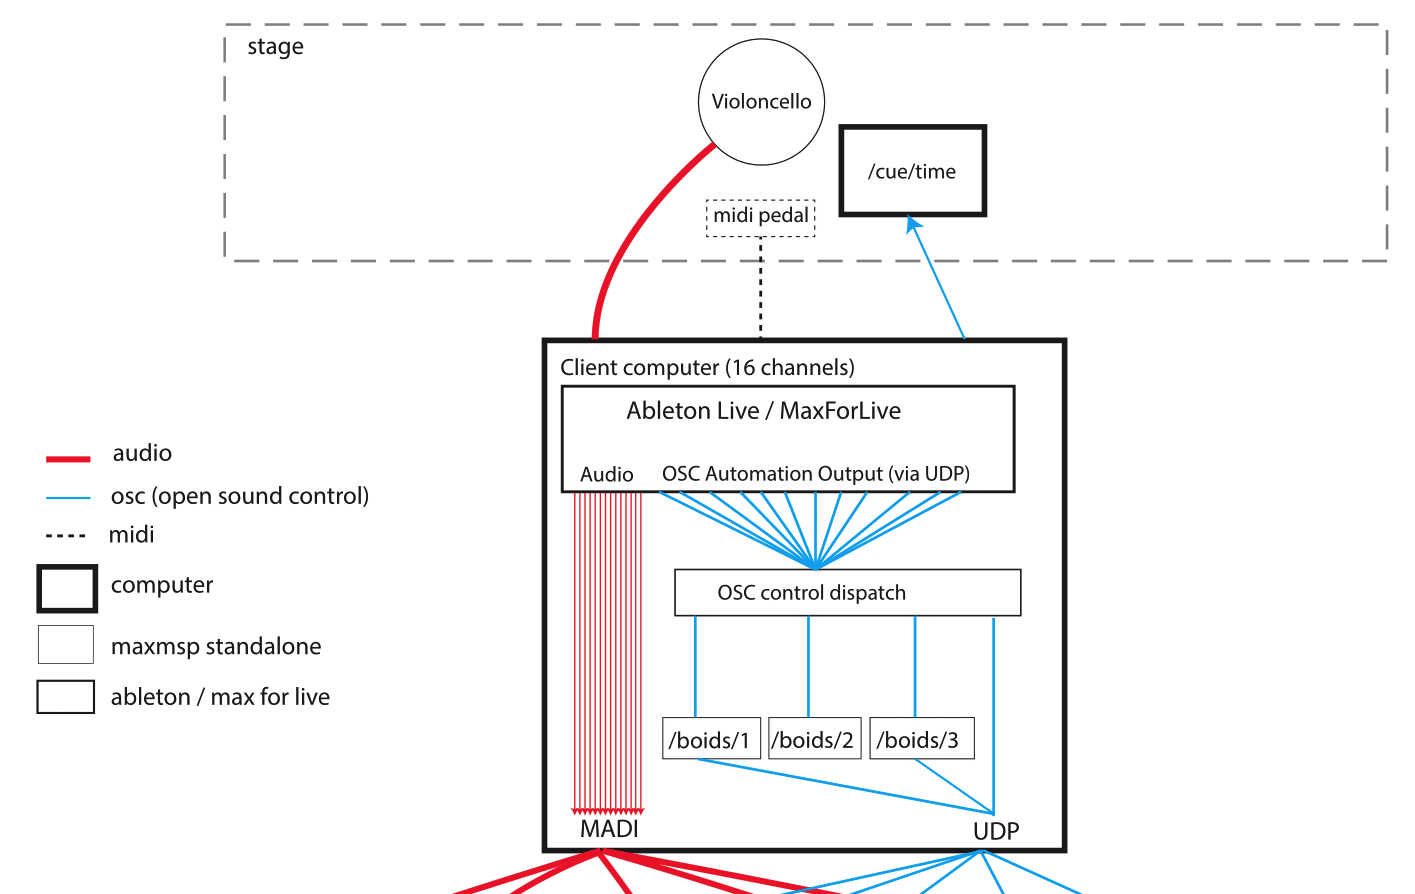
\includegraphics[keepaspectratio=true, width=\textwidth]{Notation/i/schemaInstallationFluoresce.png}
	\caption[Schéma de branchement pour la pièce \textit{Fluoresce} par Rama Gottfried]{Schéma de branchement pour la pièce \textit{Fluoresce} par Rama Gottfried}
	\label{fig:schemaInstallationFluoresce}			
\end{figure}
\begin{center}
\small \it La figure \ref{fig:schemaInstallationFluoresce} présente le schéma de câblage des différents éléments qui vont servir à l'exécution de la pièce. La performance fait intervenir un joueur de violoncelle (\textit{Violoncello}); le son produit par le violoncelle est capté et envoyé à un ordinateur (\textit{Client computer}) sur lequel est lancé la station audionumérique\footnote{\og Une station audionumérique (acronyme DAW, de l'anglais digital audio workstation) désigne […] un ensemble d'outils électroniques, conçu pour enregistrer, éditer, manipuler, créer et lire des contenus audionumériques.\fg -- Wikipédia} \textit{Ableton Live} associé au plugin \textit{MaxForLive}\footnote{MaxForLive est un plugin permettant l'intégration du logiciel Max/MSP à la station audionumérique Ableton Live. Voir plus loin pour plus de détails sur Max/MSP.}. Ableton Live répartit le signal audio sur les systèmes WFS et HOA (\textit{Wave Field Synthesis} et \textit{High Order Ambisonics}\footnote{\textit{Wave Field Synthesis} et \textit{High Order Ambisonics} sont deux systèmes de diffusion de sons spatialisés basés sur l'utilisation d'un grand nombre d'enceintes.}) via la liaison MADI\footnote{MADI (Multichannel Audio Digital Interface) est une liaison audionumérique définissant un protocole capable d'embarquer 64 canaux audio simultanément}. Le plugin MaxForLive envoie des messages OSC\footnote{Open Sound Control. Protocole de communiaction entre ordinateurs, synthéthiseurs et autres appareils. \textbf{Voir le chapitre} pour plus de détails.} \texttt{/boids/1}, \texttt{/boids/2} et \texttt{/boids/3} (directives de déclenchement d'effets sonores), via UDP, aux systèmes WFS et HOA. Le schéma de branchement complet est consultable en annexe \ref{sec:schemaInstallationFluoresceComplet} page~\pageref{sec:schemaInstallationFluoresceComplet}. L'écoute et la description de la pièce \textit{Fluoresce} sont accessibles à l'url \url{http://www.ramagottfried.com/fluoresce.html}.
\end{center}

Cette pièce met bien en place des moyens audiovisuels (un violoncelle, des ordinateurs, et deux systèmes de diffusion sonore…) pour traduire une expérience musicale; ici l'expérience est purement sonore, il n'y a pas de dimension multisensorielle. La pièce \textit{Fluoresce} est un type de musique appelée "musique mixte", c'est à dire qui mélange instruments traditionnels et Informatique.

Sur le schéma, l'ordinateur sur scène envoie le message OSC \texttt{/cue/time} au \textit{Client computer}. Le message \texttt{/cue/time} transmet un référentiel temporel permettant la synchronisation entre le jeu du violoncelliste et le \textit{Client computer}. 
Dans le cas de musique mixte, la question de la synchronisation humain/machine et du suivi de partition est centrale (voir la section suivante). 
En effet, même si une pièce de musique contemporaine peut se détacher de toutes notions de métrique, de mélodie et d'harmonie, elle admet tout de même un ordonnancement temporel des éléments la composant.
D'ailleurs, sur les partitions du XXème siècle, Jean-Yves Bosseur indique que la notation agit comme le \og déclencheur d'une chaîne d'actions et de réactions sonores \fg (\cite[121]{bosseur2005}), illustrant bien l'impératif de temporisation et de synchronisation inhérent à la musique contemporaine.

Pour finir, la présence d'un schéma de branchement au sein de la partition de \textit{Fluoresce} démontre la nécessité d'augmentation de la portée traditionnelle, qui n'est pas capable de retransmettre à la fois le contenu et l'agencement d'une pièce musicale.

\subsection{But de la notation pour la musique contemporaine}
\label{subsec:butDeLaNotation}
La notation musicale peut être distinguée en deux approches : un approche prescriptive et une approche descriptive \cite{battier2015}.

La notation prescriptive a pour but de décrire \og comment la musique doit sonner \fg.
Dans cette optique, la partition fait office de référence ou du moins de repère pour l'interprétation d'une pièce. 

La notation descriptive tente de retranscrire \og comment la musique a sonné \fg.
Ainsi, à des fins d'analyse, une pièce peut être caractérisée et fixée sur une partition.

La musique contemporaine hérite de la musique électroacoustique son caractère expérimental. Ainsi, la composition d'une telle musique s'effectue souvent à même la matière sonore, sans l'entremise de la partition.\\
Aussi, quel est l'objectif de la notation pour la musique contemporaine?\\
De nombreuses pièces électroacoustiques n'ont été notées qu'après coup par les musiciens les produisant (exemple, les truc-muches…). Ainsi, dans le cas de la musique contemporaine une approche descriptive de la notation serait à envisager.

Cependant, la partition reste l'outil privilégié du compositeur pour la communication de sa musique, et, au-delà de l'objet fini, constitue également un espace de travail.\\
Aussi, la préparation d'une pièce contemporaine par un ensemble musical se fait souvent en collaboration avec le compositeur. La partition constitue alors le support de la discussion et se voit même être modifiée pour les besoins de l'exécution de la pièce.\\
Comme le dit Carmine E. Cella, chercheur et compositeur à l'IRCAM, en parlant de l'écriture musicale : \og le créateur doit s'efforcer de trouver un compromis notationnel entre sa pensée et la réalisation pratique de sa pièce \fg.\\
L'annexe \ref{sec:refletsDeLOmbre} donne deux exemples de partitions représentant la même partie de la pièce \textit{Reflets de l'ombre} (C. E. Cella, 2013), montrant l'adaptation de la notation à des fins d'exécution.

En définitive, une troisième approche de la notation musicale pourrait se profiler, celle d'une conception \textit{évolutive} de la partition.

\subsection{Problématiques liées à la notation de la musique contemporaine}
\label{subsec:pbmatiquesMusiqueContemporaine}